\documentclass[10pt, conference, letterpaper]{IEEEtran}

\usepackage{algorithm}
\usepackage{algorithmicx}
\usepackage{algpseudocode}
\usepackage{amsfonts}
\usepackage{amsmath}
\usepackage{amssymb}
\usepackage[ansinew]{inputenc} 
\usepackage{xcolor}
\usepackage{mathtools}
\usepackage{graphicx}
\usepackage{caption}
\usepackage{subcaption}
\usepackage{import}
\usepackage{multirow}
\usepackage{cite}
\usepackage[export]{adjustbox}
\usepackage{breqn}
\usepackage{mathrsfs}
\usepackage{acronym}
%\usepackage[keeplastbox]{flushend}
\usepackage{setspace}
\usepackage{bm}
\usepackage{stackengine}

\usepackage{tikz}
\usetikzlibrary{arrows.meta, positioning, calc}

\usepackage{stfloats}

\usepackage{listings}

\lstset{%
 backgroundcolor=\color[gray]{.85},
 basicstyle=\small\ttfamily,
 breaklines = true,
 keywordstyle=\color{red!75},
 columns=fullflexible,
}%

\lstdefinelanguage{BibTeX}
  {keywords={%
      @article,@book,@collectedbook,@conference,@electronic,@ieeetranbstctl,%
      @inbook,@incollectedbook,@incollection,@injournal,@inproceedings,%
      @manual,@mastersthesis,@misc,@patent,@periodical,@phdthesis,@preamble,%
      @proceedings,@standard,@string,@techreport,@unpublished%
      },
   comment=[l][\itshape]{@comment},
   sensitive=false,
  }

\usepackage{listings}

% listings settings from classicthesis package by
% Andr\'{e} Miede
\lstset{language=[LaTeX]Tex,%C++,
    keywordstyle=\color{RoyalBlue},%\bfseries,
    basicstyle=\small\ttfamily,
    %identifierstyle=\color{NavyBlue},
    commentstyle=\color{Green}\ttfamily,
    stringstyle=\rmfamily,
    numbers=none,%left,%
    numberstyle=\scriptsize,%\tiny
    stepnumber=5,
    numbersep=8pt,
    showstringspaces=false,
    breaklines=true,
    frameround=ftff,
    frame=single
    %frame=L
}

\renewcommand{\thetable}{\arabic{table}}
\renewcommand{\thesubtable}{\alph{subtable}}

\DeclareMathOperator*{\argmin}{arg\,min}
\DeclareMathOperator*{\argmax}{arg\,max}

\def\delequal{\mathrel{\ensurestackMath{\stackon[1pt]{=}{\scriptscriptstyle\Delta}}}}

\graphicspath{{./figures/}}
\setlength{\belowcaptionskip}{0mm}
\setlength{\textfloatsep}{8pt}

\newcommand{\eq}[1]{Eq.~\eqref{#1}}
\newcommand{\fig}[1]{Fig.~\ref{#1}}
\newcommand{\tab}[1]{Tab.~\ref{#1}}
\newcommand{\secref}[1]{Section~\ref{#1}}

\newcommand\MR[1]{\textcolor{blue}{#1}}
\newcommand\red[1]{\textcolor{red}{#1}}
\newcommand{\mytexttilde}{{\raise.17ex\hbox{$\scriptstyle\mathtt{\sim}$}}}

%\renewcommand{\baselinestretch}{0.98}
% \renewcommand{\bottomfraction}{0.8}
% \setlength{\abovecaptionskip}{0pt}
\setlength{\columnsep}{0.2in}

% \IEEEoverridecommandlockouts\IEEEpubid{\makebox[\columnwidth]{PUT COPYRIGHT NOTICE HERE \hfill} \hspace{\columnsep}\makebox[\columnwidth]{ }} 

\title{NNDL project report template}

\author{Edoardo Furlan$^\dag$, Andrea Marigo$^\dag$, Francesca Zorzi$^\dag$
\thanks{$^\dag$Department of Information Engineering, University of Padova, \newline email: \texttt{\{edoardo.furlan.3, andrea.marigo.3, francesca.zorzi.3\}@studenti.unipd.it}}
} 

\IEEEoverridecommandlockouts

\newcounter{remark}[section]
\newenvironment{remark}[1][]{\refstepcounter{remark}\par\medskip
   \textbf{Remark~\thesection.\theremark. #1} \rmfamily}{\medskip}

\begin{document}

\maketitle

\begin{abstract}
  In the field of generative AI, the task of music generation is heavily conditioned by the need of training a network that not only provides notes, but is able to produce pieces of music made of a coherent sequence of notes, and may be good for the human ear.
  Inspired by Midinet \cite{Yang-2017}, our system is a conditioned Generative Adversarial Network (GAN) enhanced with a set of residual blocks and a dedicated Conditioner network that extracts features from previous bars to ensure temporal continuity.
  To produce a stable learning process, we adopt a Wasserstein loss with gradient penalty (WGAN-GP), replacing the standard binary cross-entropy. Also, the Critic (as we will call the Discriminator network, due to the new loss function) is enhanced with a Minibatch Standard Deviation layer, which provides information that helps in penalizing repetitive outputs.
  The integration of these systems is used to produce piano music from an underlying chord progression, generating coherent music.
  %\MR{This is an example abstract from a paper we wrote a couple of years ago. I would say an abstract should not be longer than $250$ words. Here, you should briefly state: 
  %\begin{enumerate}
  %\item the technical scenario/field of research and its timeliness/relevance in general (one sentence),
  %\item what you do in the report/paper and why it is important, how it advances the state of the art in its field (a few sentences), 
  %\item summarize the main and best results of your study/proposal/method (one or two sentences),
  %\item (optional) how others could benefit from your results for further research, or within commercial products (one sentence).
  %\end{enumerate}  
  %The abstract is one of the most important parts of the paper/report. You have roughly one minute to catch the reader's attention. A poor abstract may already move you towards the rejection side in the reviewer's decision process. In the abstract, 1) establish the context, 2) motivate the problem, 3) briefly describe the solution, and 4) present the main results of your work. Ideally, use one (short) sentence for each of the previously mentioned items to keep your abstract short. Overall, this should be a short summary of the whole content of your paper, including your results.}

  %\MR{See the abstract as a personal challenge for each of your papers. Finally, the abstract should contain the main message about your work, so that the reader will now what she/he can find even without reading it (as it is the case most of the times). The abstract is a mini-paper on its own and, as such, it is a major endeavor to write.}

  %\red{I suggest to write the Abstract as the very last thing. You may sketch it at the beginning, but then always finalize it at the end.}
\end{abstract}

\begin{IEEEkeywords}
Neural Networks, Convolutional Neural Networks, Generative Adversarial Networks, Symbolic-Domain Music
\end{IEEEkeywords}


\input{Intro}

% !TEX root = template.tex

\section{Related Work}
\label{sec:related_work}
Our network is based on the MidiNet architecture \cite{Yang-2017}. 
What this architecture introduced is the idea of conditioning the generation process by combining the outputs of convolutional layer of a Conditioner network to the input of the layers of the Generator.
In this way the network is able to produce music coherent with previous bars. However, while training an exact copy of the network we noted the typical struggles of GANs: the Discriminator was quickly able to distinguish real from fake music, leading to a completely random Generation process.
Our work then focused on finding ways to improve the balance between the two networks. The main idea was the modification of the loss function. As already said, the MidiNet paper opens to the possibiliy of changing to a loss that avoids vanishing gradients, which is the one we chose in our network. 

% !TEX root = template.tex

\section{Processing Pipeline}
\label{sec:processing_architecture}

A schematic represtation of the network is shown in Figure \textbf{Inserire figura}

\subsection{Generator Res-CNN and Critic CNN}
\label{sec:generator_critic_cnn}

We used a DCGAN architecture which has the objective of training a Critic CNN to distinguish between real samples and samples generated by a Generator Res-CNN, which aims at fooling the Critic.
For the generation process we used random noises $z \in \mathbb{R}^{100}$ sampled from a Normal Gaussian distribution, which are passed through a series of transposed conolutional layers and residual blocks to produce the correct output matrix representing the music bar.
The Critic CNN is a convolutional network which takes as input a music bar and outputs a single scalar value representing the "score" of the bar, i.e. how likely it is to be a real music bar.

This produces a minimax game between Generator and Critic, which ensures non-saturating gradients for both networks, due to the linearity of the Critic's output. More details about the loss structure will be explained in Section \ref{sec:wasserstein_loss}.

In order to deal with mode collapse, \cite{Yang-2017} introduced feature matching and one-sided label smoothing. After trying these ideas in our network, wefound that they were not enough to solve the problem. As a consequence, to obtain more control over the game we also introduced a minibatch discrimination block in the Critic CNN.
This block computes the standard deviation of each feature across the batch, averages it to a single scalar $s = \text{mean}_{c,h,w}(\text{std}b(I{b,c,h,w}))$ and concatenates it as an additional channel. The idea is to provide the Critic with a statistical point of view of the input samples, forcing the Generator to produce music without collapsing to one single mode.
\subsection{Conditioner Network}
\label{sec:conditioner_network}
Our network also takes the contidioning idea of \cite{Yang-2017}. The Conditioner Network is a CNN which takes as input a conditioning matrix and concatenates the output of each convolutional layer to the output of the corresponding layer of the generator, leading to an influenced generation process.



\input{signals_features}


% !TEX root = template.tex

\begin{figure*}[!t]
    \centering
    \fcolorbox{gray}{white}{%
        \resizebox{\textwidth}{!}{
            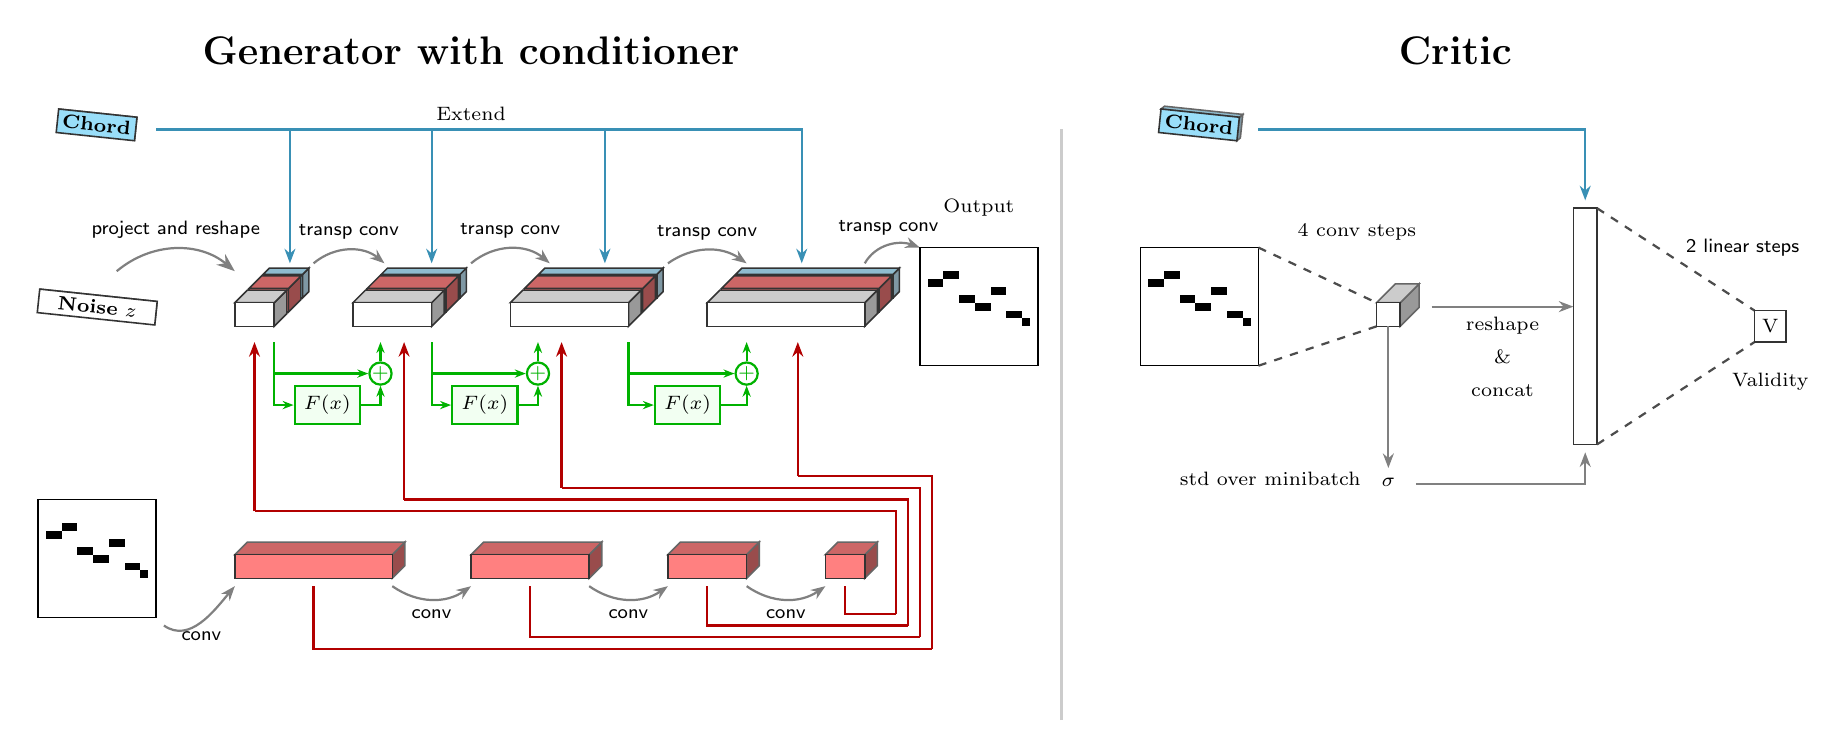
\begin{tikzpicture}[x=1cm, y=1cm, >=Stealth]

    % ==========================================
    % MACROS PER DISEGNARE I BLOCCHI E I DETTAGLI
    % ==========================================

    % Macro per i tensori 3D Args: x, y, width, height, depth, color, label_text
    \newcommand{\drawbox}[7]{
        \pgfmathsetmacro{\dx}{#5*0.4}
        \pgfmathsetmacro{\dy}{#5*0.4}
        % Right side (depth)
        \draw[fill=#6!60!black, draw=black!60, line width=0.2mm] (#1+#3,#2) -- ++(\dx,\dy) -- ++(0,#4) -- ++(-\dx,-\dy) -- cycle;
        % Top side
        \draw[fill=#6!80!black, draw=black!60, line width=0.2mm] (#1,#2+#4) -- ++(\dx,\dy) -- ++(#3,0) -- ++(-\dx,-\dy) -- cycle;
        % Front face
        \draw[fill=#6, draw=black!80, line width=0.2mm] (#1,#2) rectangle ++(#3,#4);

        % 2. Centered Text Node inside the box
        \node[text width=#3 cm, align=center, font=\scriptsize, text=black, transform shape] at (#1+#3/2, #2+#4/2) {#7};
    }

    \newcommand{\slicebox}[7]{
        % #1=x, #2=y, #3=w, #4=h, #5=slice_d, #6=shift_d, #7=color
        \pgfmathsetmacro{\xshift}{#6*0.4}
        \pgfmathsetmacro{\yshift}{#6*0.4}
        \pgfmathsetmacro{\dx}{#5*0.4}
        \pgfmathsetmacro{\dy}{#5*0.4}

        \coordinate (FBL) at (#1+\xshift, #2+\yshift); % Front Bottom Left della fetta
        % Right side
        \draw[fill=#7!60!black, draw=black!80, line width=0.2mm] (#1+\xshift+#3, #2+\yshift) -- ++(\dx,\dy) -- ++(0,#4) -- ++(-\dx,-\dy) -- cycle;
        % Top side
        \draw[fill=#7!80!black, draw=black!80, line width=0.2mm]  (#1+\xshift, #2+\yshift+#4) -- ++(\dx,\dy) -- ++(#3,0) -- ++(-\dx,-\dy) -- cycle;
        % Front face
        \draw[fill=#7, draw=black!80, line width=0.2mm] (FBL) rectangle ++(#3,#4);
    }

    % 3. Macro per il tensore concatenato (Bianco + Rosso + Blu)
    \newcommand{\drawsplitbox}[6]{
        % #1=x, #2=y, #3=w, #4=h, #5=d, #6=label    
        % Retro: Ultimi 12 canali (Blu)
        \slicebox{#1}{#2}{#3}{#4}{0.2*#5}{0.9*#5}{myblue}
        % Centro: Successivi 256 canali (Rossi)
        \slicebox{#1}{#2}{#3}{#4}{0.4*#5}{0.45*#5}{myred}
        % Fronte: Primi 256 canali (Bianchi)
        \slicebox{#1}{#2}{#3}{#4}{0.4*#5}{0}{mywhite}
        % Testo sulla faccia frontale
        \node[text width=#3 cm, align=center, font=\scriptsize, text=black, transform shape] at (#1+#3/2, #2+#4/2) {#6};
    }

    % 4. Macro per il Residual Layer
    \newcommand{\resblock}[3]{
    % #1=startX, #2=startY, #3=endX
    \pgfmathsetmacro{\midX}{(#1+#3)/2}
    \pgfmathsetmacro{\plusY}{#2-0.4}
    \pgfmathsetmacro{\fY}{#2-0.8}

    % Box F(x) - Componenti verdi, testo nero
    \node[draw=mygreenLine, fill=mygreen!10, thick, text=black, minimum width=0.6cm, minimum height=0.4cm, font=\scriptsize, align=center] (fx) at (\midX, \fY) {$F(x)$};
    % Nodo Sommatore (+)
    \node[draw=mygreenLine, circle, inner sep=0pt, minimum size=0.25cm, thick, text=mygreenLine, font=\scriptsize] (plus) at (#3, \plusY) {$+$};

    % Rami con frecce più piccole e raffinate (scale=0.7)
    \draw[-{Stealth[scale=0.6]}, draw=mygreenLine, thick] (#1, #2) |- (fx.west);
    \draw[-{Stealth[scale=0.6]}, draw=mygreenLine, thick] (#1, #2) |- (plus.west);
    \draw[-{Stealth[scale=0.6]}, draw=mygreenLine, thick] (fx.east) -| (plus.south);
    \draw[-{Stealth[scale=0.6]}, draw=mygreenLine, thick] (plus.north) -- (#3, #2);
    }

    % Macro per il "piano roll" (i quadratini neri)
    \newcommand{\pianoroll}[2]{
        % Background box to contain the notes
        \draw[fill=white, draw=black, line width=0.2mm] (#1, #2) rectangle ++(1.5, 1.5);
        % Note blocks
        \fill[black] (#1+0.1, #2+1.0) rectangle ++(0.2, 0.1);
        \fill[black] (#1+0.3, #2+1.1) rectangle ++(0.2, 0.1);
        \fill[black] (#1+0.5, #2+0.8) rectangle ++(0.2, 0.1);
        \fill[black] (#1+0.7, #2+0.7) rectangle ++(0.2, 0.1);
        \fill[black] (#1+0.9, #2+0.9) rectangle ++(0.2, 0.1);
        \fill[black] (#1+1.1, #2+0.6) rectangle ++(0.2, 0.1);
        \fill[black] (#1+1.3, #2+0.5) rectangle ++(0.1, 0.1);
    }

    % Colori personalizzati per i blocchi
    \colorlet{myblue}{cyan!40}
    \colorlet{myred}{red!50}
    \colorlet{mygreen}{green!50}
    \colorlet{mywhite}{white}

    % Colori personalizzati (più scuri) per le linee e le frecce
    \colorlet{myblueLine}{cyan!70!black}
    \colorlet{myredLine}{red!70!black}
    \colorlet{mygreenLine}{green!70!black}

    % ==========================================
    % PARTE SINISTRA: CONDITIONER E GENERATOR
    % ==========================================

    % --- Titoli ---
    \node at (6, 9) {\Large \textbf{Generator with conditioner}};

    % ----------- MAIN PIPELINE -------------
    % Noise z (ruotato)
    \begin{scope}[rotate around={-6:(0,1)}]
        \drawbox{0}{5.7}{1.5}{0.3}{0}{mywhite}{\textbf{Noise $z$}};
    \end{scope}
    \draw[-{Stealth}, thick, gray] (1.5, 6.2) to[out=40, in=140] node[midway, above, text=black] {\scriptsize \textsf{project and reshape}} (3.0, 6.2);

    % First tensor: 524x1x2 (Utilizziamo la nuova \drawsplitbox)
    \drawsplitbox{3}{5.5}{0.5}{0.3}{1}{}
    \resblock{3.5}{5.3}{4.85}
    \draw[-{Stealth[scale=0.8]}, thick, gray] (4, 6.3) to[out=40, in=140] node[midway, above, text=black] {\scriptsize \textsf{transp conv}} (4.9, 6.3);

    % Second tensor: 524x1x4
    \drawsplitbox{4.5}{5.5}{1}{0.3}{1}{}
    \resblock{5.5}{5.3}{6.85}
    \draw[-{Stealth[scale=0.8]}, thick, gray] (6, 6.3) to[out=40, in=140] node[midway, above, text=black] {\scriptsize \textsf{transp conv}} (7, 6.3);

    % Third tensor: 524x1x8
    \drawsplitbox{6.5}{5.5}{1.5}{0.3}{1}{}
    \resblock{8}{5.3}{9.5}
    \draw[-{Stealth[scale=0.8]}, thick, gray] (8.5, 6.3) to[out=35, in=145] node[midway, above, text=black] {\scriptsize \textsf{transp conv}} (9.5, 6.3);

    % Fourth tensor: 524x1x16
    \drawsplitbox{9}{5.5}{2}{0.3}{1}{}
    \draw[-{Stealth[scale=0.8]}, thick, gray] (11, 6.3) to[out=60, in=160] node[midway, above, text=black] {\scriptsize \textsf{transp conv}} (11.7, 6.5);

    % Final Piano Roll
    \pianoroll{11.7}{5}
    \node at (12.45, 7) {\scriptsize Output};

    % ----------- CONDITION 1D -------------    
    \begin{scope}[rotate around={-6:(0,1)}]
        \drawbox{0}{8}{1}{0.3}{0}{myblue}{\textbf{Chord}};
    \end{scope}

    \draw[-{Stealth[scale=0.8]}, thick, myblueLine] (2, 8) -| (3.7, 6.3);
    \draw[-{Stealth[scale=0.8]}, thick, myblueLine] (2, 8) -| (5.5, 6.3);
    \draw[-{Stealth[scale=0.8]}, thick, myblueLine] (2, 8) -| (7.7, 6.3);
    \draw[-{Stealth[scale=0.8]}, thick, myblueLine] (2, 8) -| (10.2, 6.3);

    \node at (6, 8.2) {\scriptsize Extend};

    % ----------- CONDITION 2D -------------
    \pianoroll{0.5}{1.8}
    \draw[-{Stealth[scale=0.8]}, thick, gray] (2.1, 1.7) to[out=-35, in=-130] node[midway, below, text=black] {\scriptsize \textsf{conv}} (3, 2.2);

    \drawbox{3}{2.3}{2}{0.3}{0.4}{myred}{}
    \draw[-{Stealth[scale=0.8]}, thick, gray] (5, 2.2) to[out=-35, in=-145] node[midway, below, text=black] {\scriptsize \textsf{conv}} (6, 2.2);
    \drawbox{6}{2.3}{1.5}{0.3}{0.4}{myred}{}
    \draw[-{Stealth[scale=0.8]}, thick, gray] (7.5, 2.2) to[out=-35, in=-145] node[midway, below, text=black] {\scriptsize \textsf{conv}} (8.5, 2.2);
    \drawbox{8.5}{2.3}{1}{0.3}{0.4}{myred}{}
    \draw[-{Stealth[scale=0.8]}, thick, gray] (9.5, 2.2) to[out=-35, in=-145] node[midway, below, text=black] {\scriptsize \textsf{conv}} (10.5, 2.2);
    \drawbox{10.5}{2.3}{0.5}{0.3}{0.4}{myred}{}

    % |- arrows
    \draw[thick, myredLine] (10.75, 2.2) |- (11.40, 1.85);
    \draw[thick, myredLine] (9, 2.2) |- (11.55, 1.7);
    \draw[thick, myredLine] (6.75, 2.2) |- (11.7, 1.55);
    \draw[thick, myredLine] (4, 2.2) |- (11.85, 1.40);

    % |- arrows
    \draw[thick, myredLine] (11.40, 1.85) |- (3.25, 3.15);
    \draw[thick, myredLine] (11.55, 1.7) |- (5.15, 3.30) ;
    \draw[thick, myredLine] (11.7, 1.55) |- (7.15, 3.45);
    \draw[thick, myredLine] (11.85, 1.40) |- (10.15, 3.60);

    % final arrows
    \draw[-{Stealth[scale=0.8]}, thick, myredLine] (3.25, 3.15) -- (3.25, 5.3);
    \draw[-{Stealth[scale=0.8]}, thick, myredLine] (5.15, 3.30) -- (5.15, 5.3);
    \draw[-{Stealth[scale=0.8]}, thick, myredLine] (7.15, 3.45) -- (7.15, 5.3);
    \draw[-{Stealth[scale=0.8]}, thick, myredLine] (10.15, 3.60) -- (10.15, 5.3);

    % ==========================================
    % SEPARATORE CENTRALE
    % ==========================================
    \draw[line width=0.4mm, gray!40] (13.5, 0.5) -- (13.5, 8);

    % ==========================================
    % PARTE DESTRA: DISCRIMINATOR
    % ==========================================

    \node at (18.5, 9) {\Large \textbf{Critic}};

    % 1. Input Piano Roll
    \pianoroll{14.5}{5}

    % 2. Converging dashed lines for Conv Layers
    \draw[dashed, thick, black!70] (16.0, 6.5) -- (17.5, 5.8);
    \draw[dashed, thick, black!70] (16.0, 5.0) -- (17.5, 5.5);
    \node at (17.25, 6.7) {\scriptsize 4 conv steps};

    % 3. Conv Feature Map Block (256x1x1)
    \drawbox{17.5}{5.5}{0.3}{0.3}{0.6}{mywhite}{}

    % 4. Minibatch Standard Deviation (sigma)
    \draw[-{Stealth[scale=0.8]}, thick, gray] (17.65, 5.5) -- (17.65, 3.7) node[below, text=black] {\scriptsize $\sigma$};
    \node[anchor=south] at (16.15, 3.35) {\scriptsize std over minibatch};

    % 5. Chord Vector Condition
    \begin{scope}[shift={(14, 0)}] % Trasla il blocco in orizzontale, allineandolo al Critic
        \begin{scope}[rotate around={-6:(0,1)}] % Usa lo stesso identico asse di rotazione del lato sinistro
            \drawbox{0}{8}{1}{0.3}{0.1}{myblue}{\textbf{Chord}};
        \end{scope}
    \end{scope}

    % 6. Reshape and Concat Arrows
    % \draw[-{Stealth[scale=0.8]}, thick, gray] (18.2, 5.75) -- (20, 5.75) node[midway, below, text=black] {\scriptsize reshape \\ \& \\ concat};
    \draw[-{Stealth[scale=0.8]}, thick, gray] (18.2, 5.75) -- (20, 5.75) node[midway, below, text=black, align=center] {\scriptsize reshape \\ \scriptsize\& \\ \scriptsize concat};
    \draw[-{Stealth[scale=0.8]}, thick, myblueLine] (16, 8) -| (20.15, 7.1);
    \draw[-{Stealth[scale=0.8]}, thick, gray] (18, 3.5) -| (20.15, 3.9);

    % 7. Combined Flattened Vector (269 dims = 256 + 1 + 12)
    \drawbox{20}{4.0}{0.3}{3.0}{0}{mywhite}{}

    % 8. Fully Connected Convergence
    \draw[dashed, thick, black!70] (20.3, 7.0) -- (22.3, 5.7);
    \draw[dashed, thick, black!70] (20.3, 4.0) -- (22.3, 5.3);
    \node at (22.15, 6.5) {\scriptsize \textsf{2 linear steps}};

    % 9. Output Validity Node
    \drawbox{22.3}{5.3}{0.4}{0.4}{0}{mywhite}{V};
    \node at (22.5, 4.8) {\scriptsize Validity};

\end{tikzpicture}
        }
    }
    \caption{Model architecture: Generator with conditioner (left) and Critic (right).}
    \label{fig:model_architecture}
\end{figure*}

\section{Learning Framework}
\label{sec:learning_framework}

\subsection{Model Architecture}
\label{sec:model_architecture}

The noise given as inpute to the Generator $G$ is first processed throught two fully-connected layers, of $1024$ and $512$ neurons respectively, and then reshaped in a tensor of shape $(1, 256, 1, 2)$.
This is then followed by four convolutional layers, where at each stage a chord embedding $c \in \mathbb{R}^{12}$ is concatenated to the feature maps. The first three layers use filters of shape $(1, 2)$ and stride $2$, doubling the temporal dimesion at each step. To avoid vanishing gradients and ensure more stability, we integrated a Residual Block after each upsampling layer.
Finally, a transposed convolution with kernel $128 \times 1$ followed by a sigmoid activation procues the final bar of shape $128 \times 16$.

The Conditioner stricly follows the structure described in \cite{Yang-2017}. The aim is to enforce temporal continuity by conditioning the Generator on the previous bar. Its structure mirrors the one of the Generator. The output of each layer is concatenated with the corresponding Generator step along with its upsampling path.

Finally, the Critic is composed of four convolutional layers, with filters of shape $(4, 4)$ and stride $2$. The idea is to progressiveli extract features from the input bar, reducing spatial dimension from $128 \times 16$ to $1 \times 1$ with $256$ channels. Additnionally, we included a Minibatch Standard Deviation layer after the final convolutional stage. Its aim is to provide the network with a statistical information about the batch diversity, resulting in a scalar that is concatenated with the extracted features. These are then flattened, concatenated to the chord embedding and passed through a final fully connected layer, which outputs a single scalar value. Here we removed the Sigmoid activation, as it was not needed for the loss function we used.
\subsection{Wasserstein Loss and Gradient Penalty}
\label{sec:wasserstein_loss}

To address the vanishing gradient problem, we adopted the Wasserstein GAN with Gradient Penalty (WGAN-GP) as explained in \cite{Gulrajani-2017}.
The idea is to minimize the Wasserstein distance between the real distribution $P_r$ and the generated distribution $P_g$.
This distance is estimated via a 1-Lipschitz function $D$ (the Critic):
\begin{equation}
    W(P_r, P_g) = \sup_{\|D\|_L \leq 1} \mathbb{E}_{x \sim P_r}[D(x)] - \mathbb{E}_{\tilde{x} \sim P_g}[D(\tilde{x})]
\end{equation}
where $D(x)$ is the scalar output of the Critic, that can be seen as a score given to the generated music.

The losses for generator and Critic are computed as:
    
\begin{equation}
    L_D = \mathbb{E}_{\tilde{x} \sim P_g}[D(\tilde{x})] - \mathbb{E}_{x \sim P_r}[D(x)]
\end{equation}
\begin{equation}
    L_G = -\mathbb{E}_{\tilde{x} \sim P_g}[D(\tilde{x})]
\end{equation}

By minimizing $L_D$ the Critic learns to provide an increasingly acurate estimation of the Wasserstein distance. On the other hand, by maximizing $L_G$ the Generator learns to produce music that receives higher scores, effectively pushing $P_g$ closer to $P_r$.

Note that the Sigmoid activation is removed from the output of the Critic, allowing the scores to grow linearly and continuously providing useful gradients.


Regarding the Gradient Penalty, it is introduced to enforce the Lipschitz constraint on the Critic, acting as a regularization term on the gradient norm. The total loss of the Critic is then computed as:
\begin{equation}
    \begin{split}
        L = & \underbrace{\mathbb{E}_{\tilde{x} \sim P_g}[D(\tilde{x})] - \mathbb{E}_{x \sim P_r}[D(x)]}_{\text{Wasserstein Loss}}                                         \\
            & + \underbrace{\lambda \mathbb{E}_{\hat{x} \sim P_{\hat{x}}} \left[ \left( \|\nabla_{\hat{x}} D(\hat{x})\|_2 - 1 \right)^2 \right]}_{\text{Gradient Penalty}}
    \end{split}
\end{equation}

Note that $\hat{x}$ is a sampled taken from a random interpolation between real and fake samples. It can be seen as a random point along the line connecting the two distributions. This forces the Discriminator to keep small gradients along the trajectories connecting real and fake samples.

\subsection{Hyperparameter tuning}
The training was influenced mainly by three hyperparameters:
\begin{enumerate}
    \item \textbf{Gradient penalty coefficient ($\lambda$):} This parameter was never modified and was always set to $10.0$ as in the original paper.
    \item \textbf{Feature matching weight ($w_{fm}$):} As a validation metric we also used the Feature Matching Loss. The idea of this metric is to force the Generator to produce music that matches the statistics of the real data, as perceived by the Critic's intermediate layers. It is used to modify the total loss of the Generator:
    \begin{equation}
        \begin{split}
            L_G &= L_{adv} + w_{fm} \cdot L_{fm} \\
            \text{where } L_{adv} &= -\mathbb{E}_{\tilde{x} \sim P_g}[D(\tilde{x})] \\
            L_{fm} &= \| \mathbb{E}_{x \sim P_r} [f(x)] - \mathbb{E}_{\tilde{x} \sim P_g} [f(\tilde{x})] \|_2^2
        \end{split}
    \end{equation}
    where $f(\cdot)$ represents the feature extractions from the Critic's convolutional layers and $w_{fm}$ is the \textit{feature matching weight}.
    Varying this parameter allows us to control the balance between statistical accuracy and melodic variety.
    \item \textbf{Number of critic steps per generator step ($n_c$):} This parameter was fundamental after the change of loss function and critic structure, as it allowed us to balance the training of the two networks. We noticed that a value between 3 and 5 was optimal for the training, to allow the critic to learn enough to provide useful gradients to the generator, which otherwise tended to collapse
\end{enumerate}
\label{sec:hyperparameter_tuning}

% !TEX root = template.tex

\section{Results}
\label{sec:results}

The results we show span the various architectures and methods we tried during the course of the project.

\subsection{Baseline Model with BCE loss}
In this first experiment we trained the baseline model with BCE loss. 
In Fig.~\ref{fig:accuracy_bce} we show the curves of the accuracy of the Discriminator. We can see that after just a few epochs this curve directly went to 1, meaning that the Generator was never able to produce valid bars of music.

\begin{figure}[!h]
    \centering
    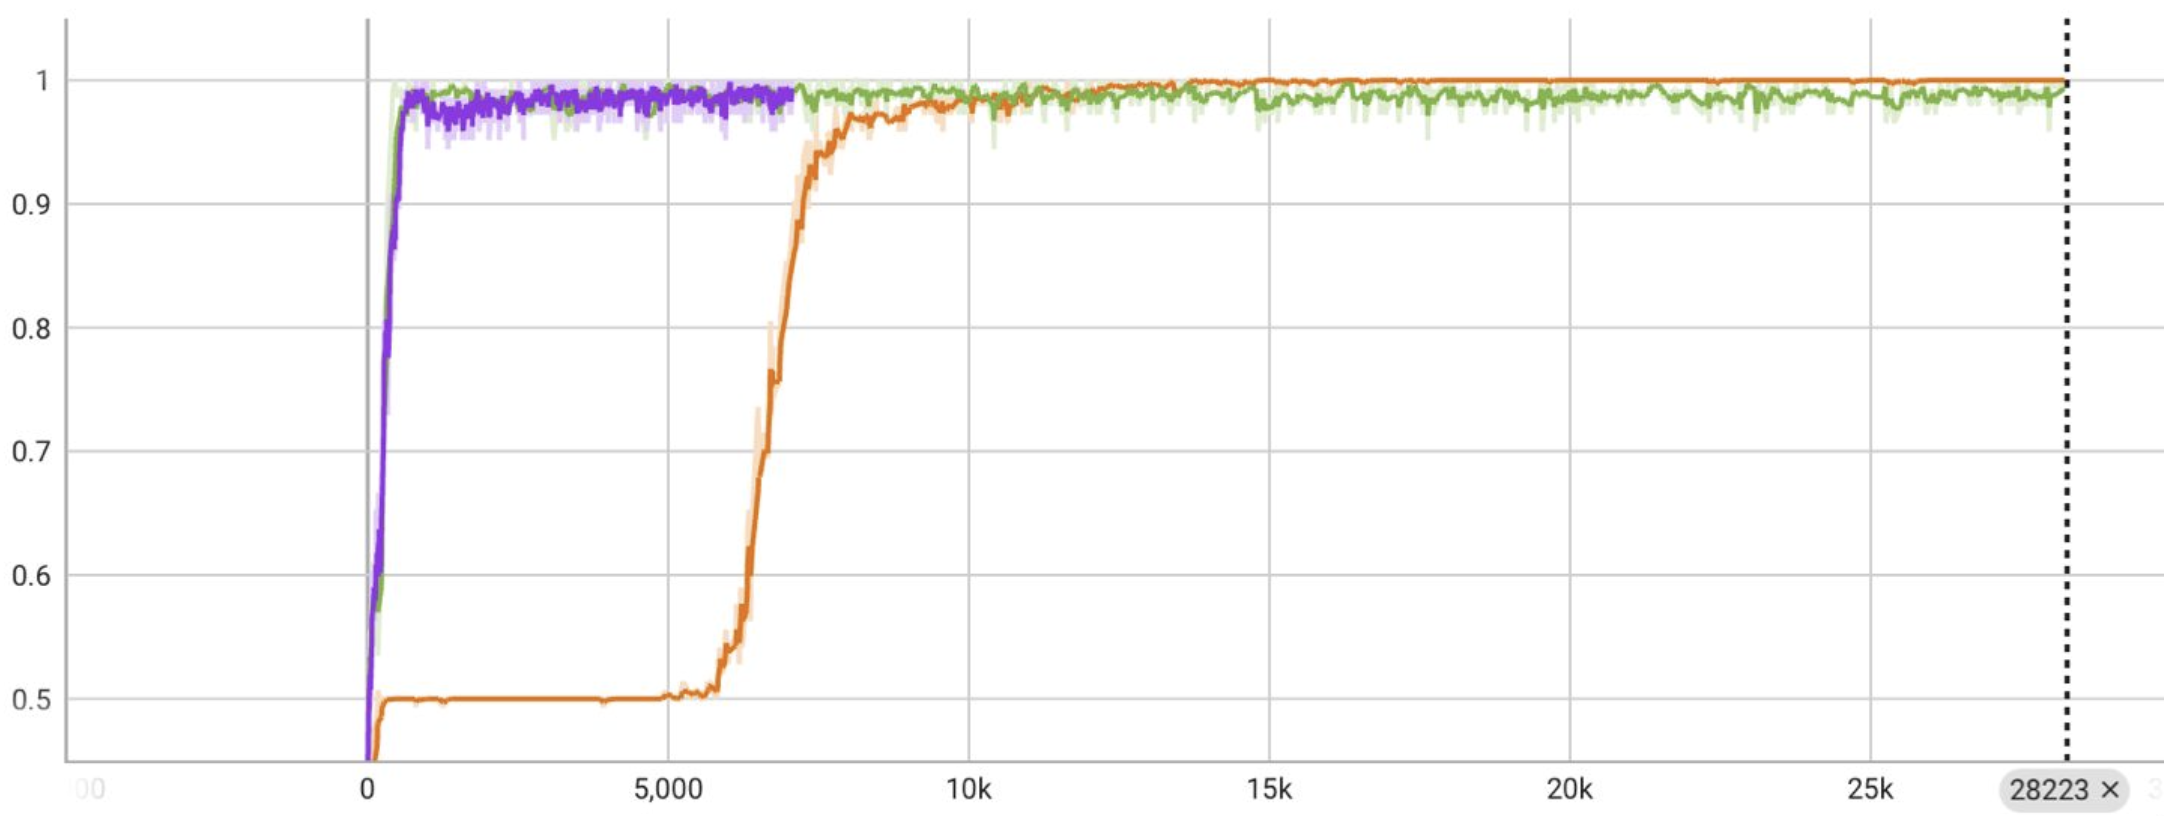
\includegraphics[width=\linewidth]{images/accuracy_BCE.png}
    \caption{Discriminator accuracy during the baseline training with BCE loss. The rapid convergence to 1 indicates that the Generator was immediately outperformed, leading to vanishing gradients.}
    \label{fig:accuracy_bce}
\end{figure}

The most delayed curve is the one corresponding to the introduction of the residual layers. Here the accuracy was able to stay around 0.5 for a few epochs, but then eventually collapsed to 1. At this point, the music produced was completely random.

\subsection{Improved Model with WGAN-GP loss}
The next step was the introduction of the WGAN-GP loss. Now, additionally to the generator and critic losses, we also tracked the \textit{Wasserstein distance estimation} and the \textit{feature matching loss}.

The idea of the first metric is that it should slowly decrease and stabilise towards zero, indicating indistinguishable distributions. Too high values indicate a too strong Critic, while too low negative values may indicate mode collapse, as the Critic is assigning too high values to the generated music

Regarding the feature matching loss, this also should slowly decrease towards low values, as it shows that the Generator is able to reproduce correctly the statistics of the real distribution. We first started with a weight of $5.0$, but gradually decrised to $0.1$ as we noticed that high values were favoring the model in reproducing average dataset statistics over diverse music, always leading to similar patterns (mode collapse).
This means that in. the last trainings this metric was less used.

At this point, even if the game seemed more balanced, the Generator was always able to produce music that fooled the Discriminator, leading to an early mode collapse.
It can be intersting to see how the loss of the generator always seemed to stay close to 0, with the critic loss being the one that fluctuated more. Looking at the produced music, we noticed that this was probably an indication of the Generator producing the same pattern over and over again, a clear signal of mode collapse.
In Fig.~\ref{fig:g_loss_collapse} and Fig.~\ref{fig:d_loss_collapse} are shown the behaviour of the two losses during training.

\begin{figure}[!h]
    \centering
    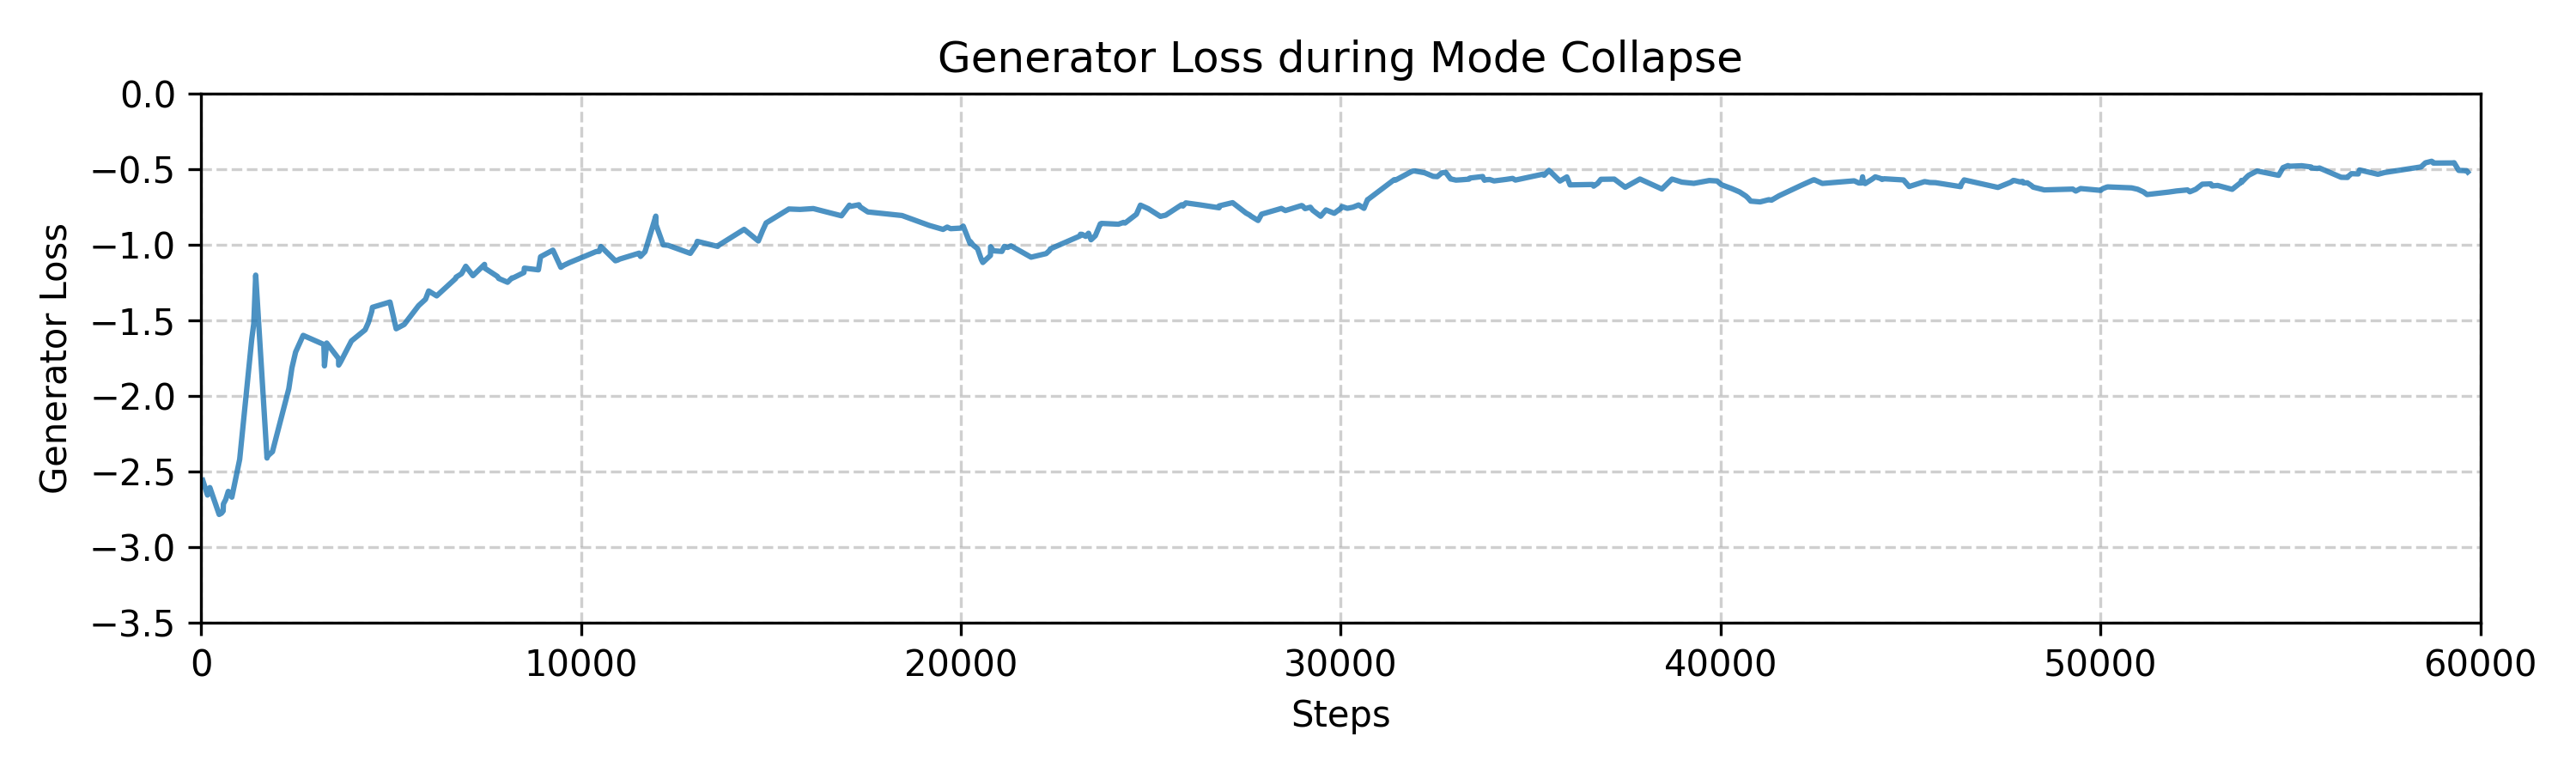
\includegraphics[width=0.9\linewidth]{images/g_loss_collapse.png}
    \caption{Generator loss curve. It remains relatively stable and close to zero.}
    \label{fig:g_loss_collapse}
\end{figure}

\begin{figure}[!h]
    \centering
    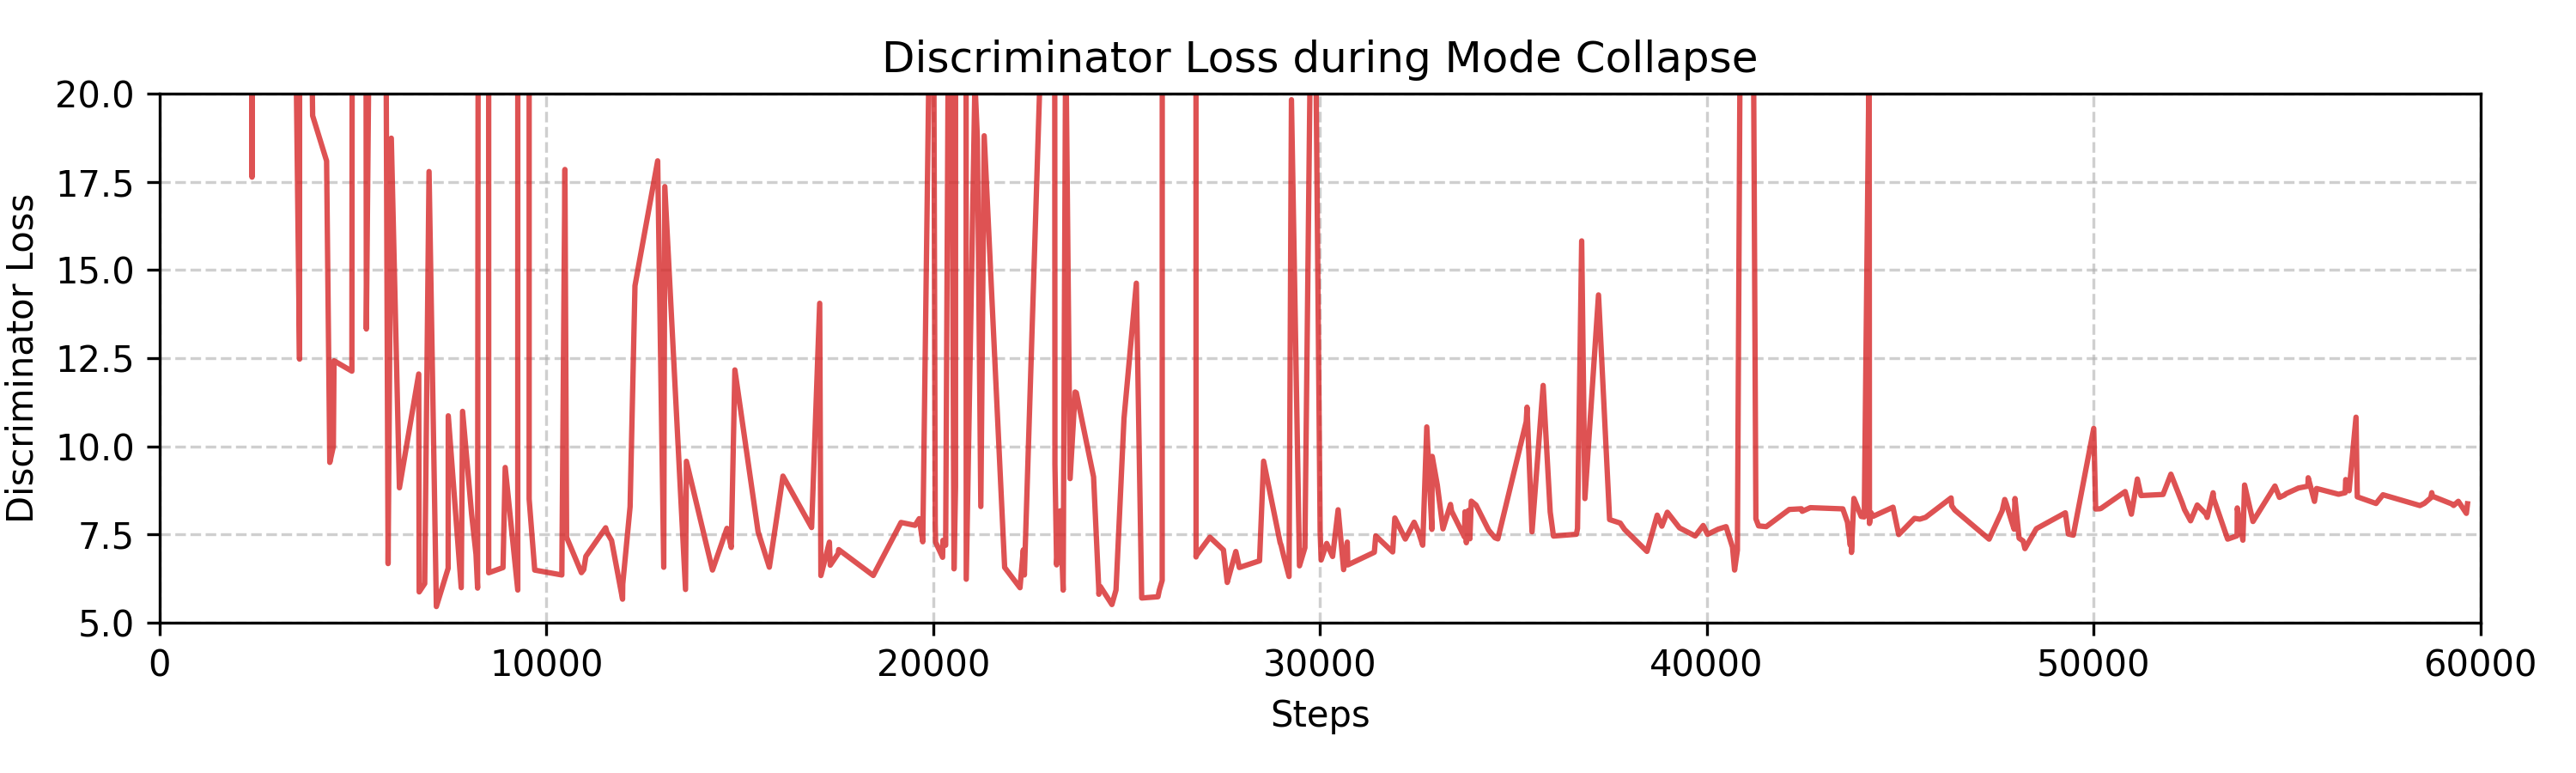
\includegraphics[width=0.9\linewidth]{images/d_loss_collapse.png}
    \caption{Discriminator loss curve. The zoom on the [0, 20] range allows to observe the spikes and fluctuations with respect to the Generator loss.}
    \label{fig:d_loss_collapse}
\end{figure}

Additionally, we also tried to produce some music at this point, as shown in Fig.~\ref{fig:piano_roll_collapse}.  The main pattern is clearly a single set of close notes continuously repeated.
\begin{figure}[!h]
    \centering
    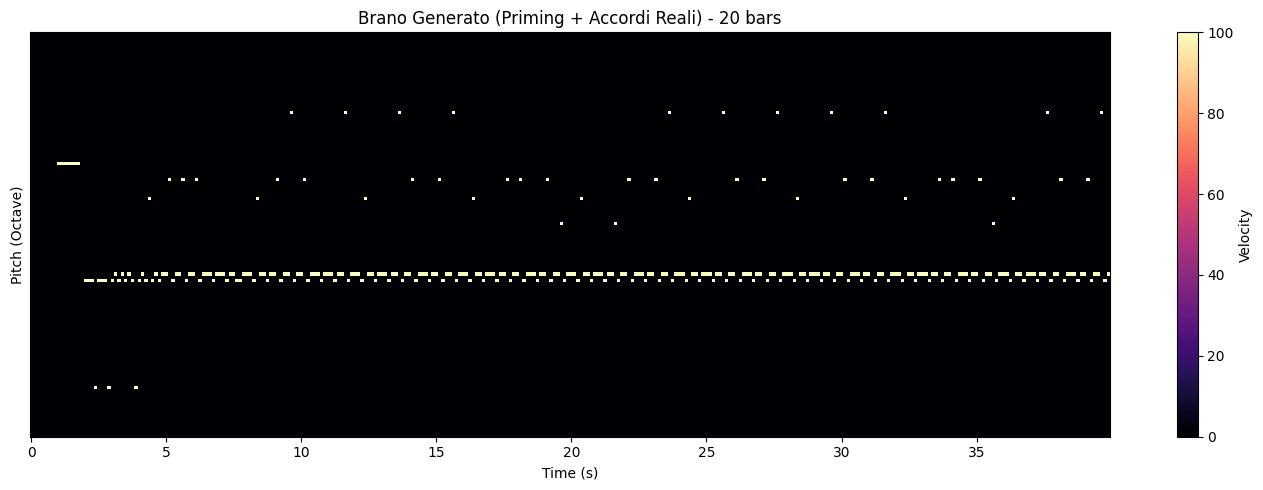
\includegraphics[width=0.9\linewidth]{images/piano_roll_collapse.jpeg}
    \caption{Generated piano roll on one of the test music.}
    \label{fig:piano_roll_collapse}
\end{figure}

\subsection{Improved Critic with minibatch std}

At this point we tried to refine the Critic's architecture as the collapsing problem was probably caused by its inability in extracting meaningful features from the produced music. We modified it into a deeper network, adding the stages we explained in \ref{sec:model_architecture}, with the objective of allowing it to extract more complex features from the music.
Additionally, to force the Generator to produce more diverse music, we tried adding the minibatch standard deviation layer. This combination led to a more active learning curve regarding the Generator and Discriminator losses and an overall more stable behaviour of the Wasserstein distance.
Here we also introduced the possibility for the Critic to perform a predefined number of updates for each update of the Generator, which allowed us to control more the balance between the two networks. In this final training it was se to $5$.
\begin{figure}[!h]
    \centering
    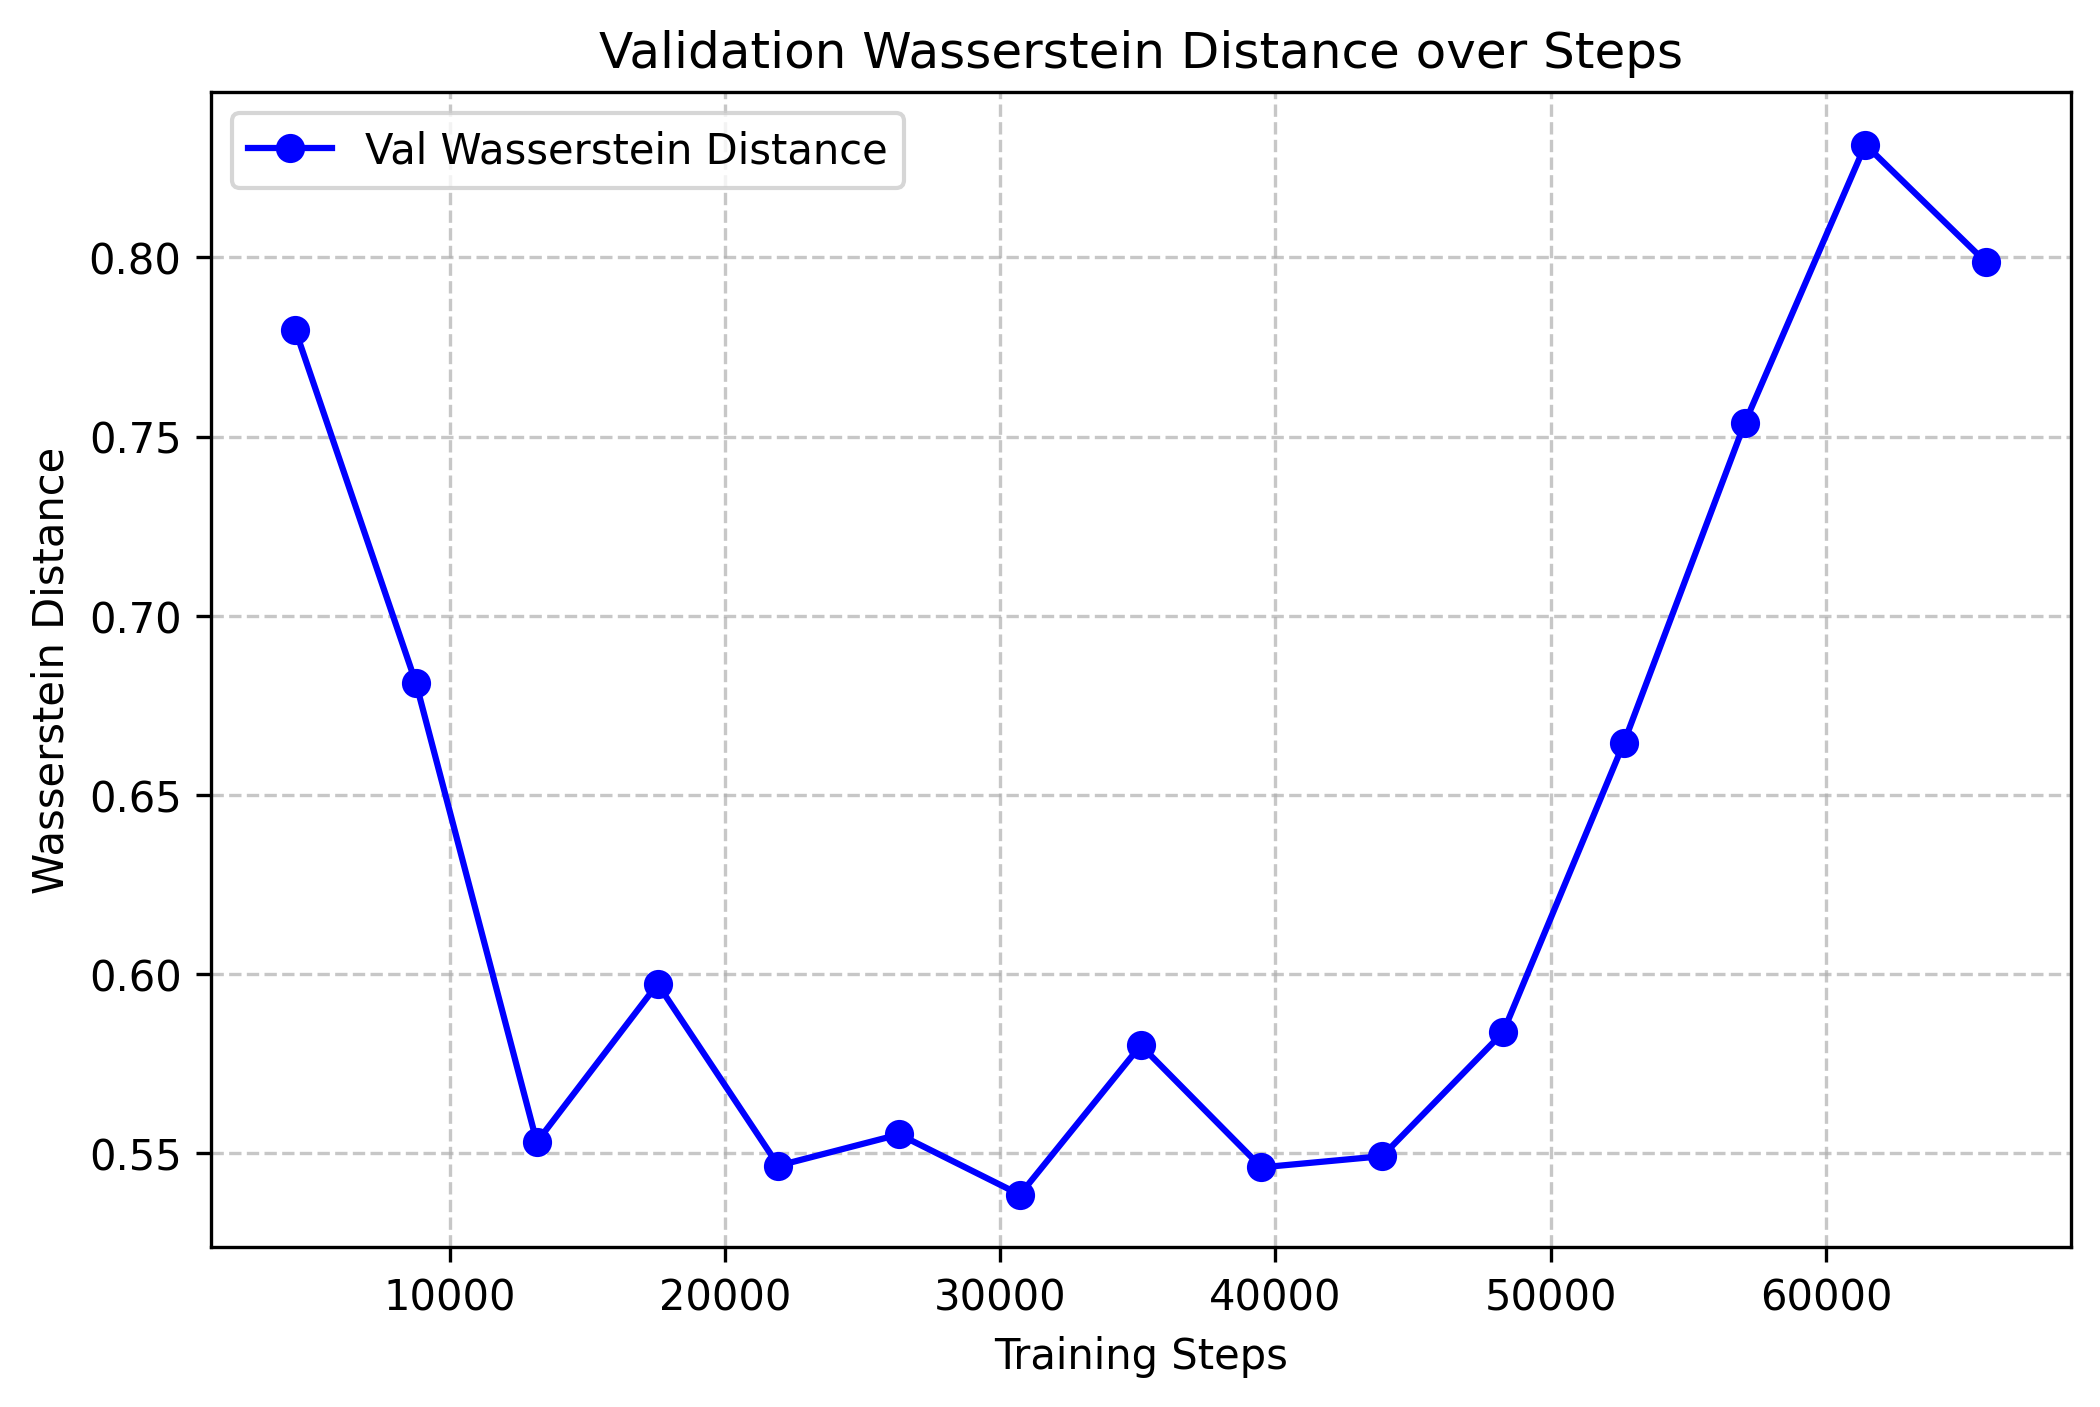
\includegraphics[width=0.7\linewidth]{images/val_w_distance.png}
    \caption{Validation Wasserstein distance during training. The initial decrease shows the model learning the distribution, while the subsequent increase suggests a potential imbalance between the Generator and the Critic.}
    \label{fig:val_w_distance}
\end{figure}

Shown in Fig.~\ref{fig:val_w_distance}, is actually the behaviour of this metric on the validation set. It reveals an interesting training dynamic. 
This training is done for 15 epochs, with the feature matching weight set to $0$, as we noticed it was not providing anymore useful results.
Initially, the distance decreases, indicating that the Generator is successfully learning to approximate the real data distribution. 
However, after approximately 40,000 steps, this curve tends to increase, suggesting that the Critic is becoming significantly more effective than the Generator.
This result shows that the model is capable of learning the real dynamics, but probably some fine tuning on the hyperparameters is still needed to reach a stable qeuilibrium and allow for longer trainings.
The results that we show in the following figures are obtained with the model at a low point on the validation curve of the validation Wasserstein distance.

\begin{figure*}[!t]
    \centering
    \begin{subfigure}{0.48\textwidth}
        \centering
        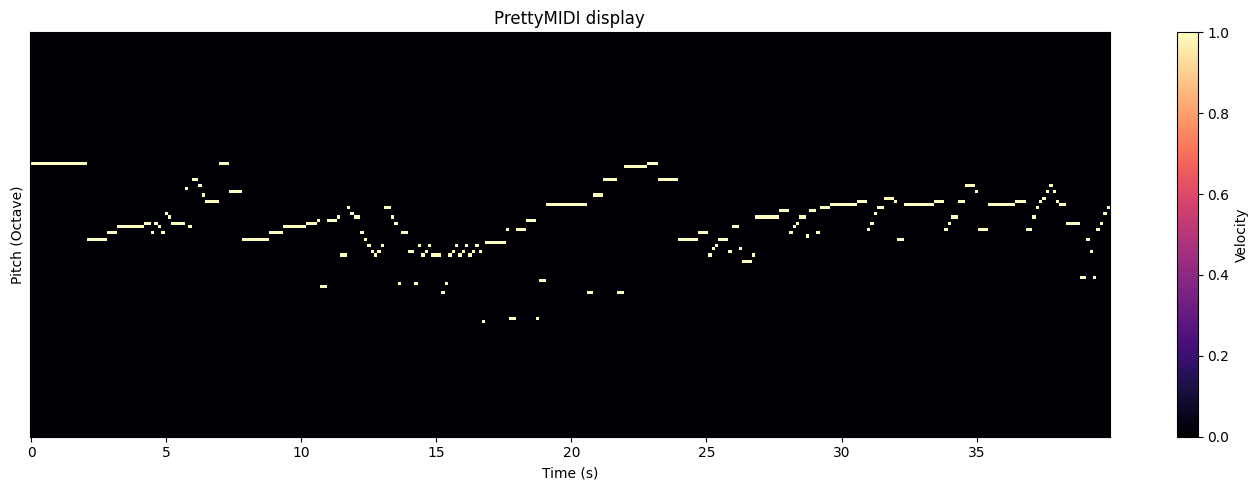
\includegraphics[width=\linewidth]{images/output_true.png}
        \caption{Ground truth sample 1 from the MAESTRO dataset.}
        \label{fig:output_true_1}
    \end{subfigure}
    \hfill
    \begin{subfigure}{0.48\textwidth}
        \centering
        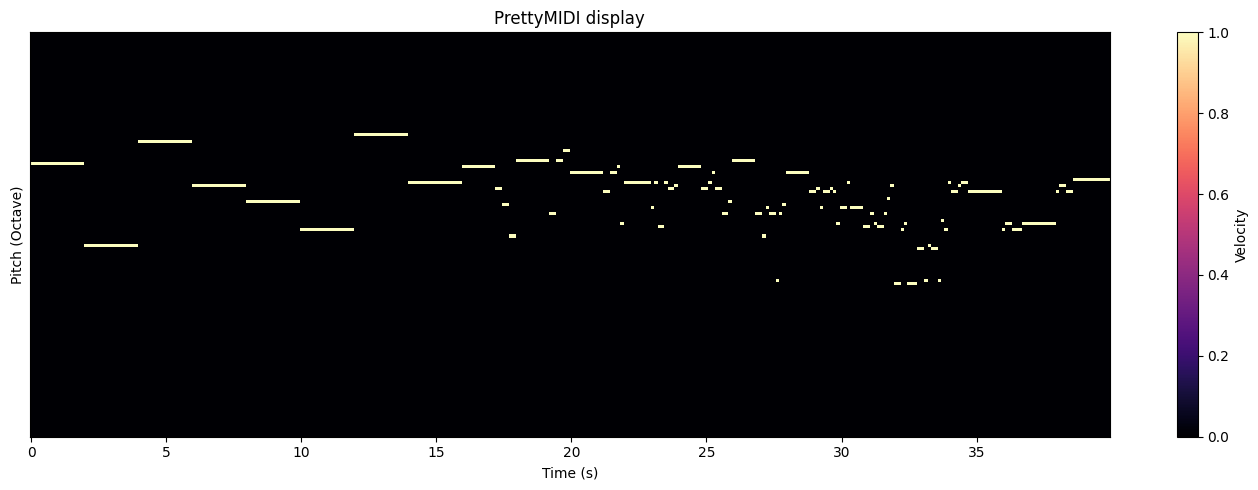
\includegraphics[width=\linewidth]{images/output_generated.png}
        \caption{Sample 1 generated by our final PianoGAN model.}
        \label{fig:output_generated_1}
    \end{subfigure}
    
    \vspace{0.4cm}
    
    \begin{subfigure}{0.48\textwidth}
        \centering
        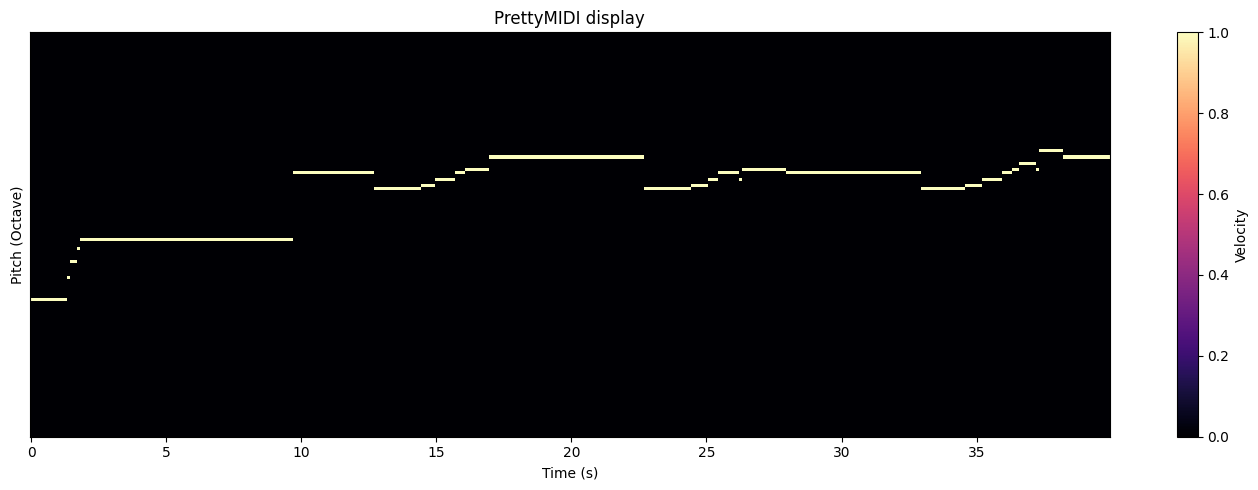
\includegraphics[width=\linewidth]{images/output_true_2.png}
        \caption{Ground truth sample 2 from the MAESTRO dataset.}
        \label{fig:output_true_2}
    \end{subfigure}
    \hfill
    \begin{subfigure}{0.48\textwidth}
        \centering
        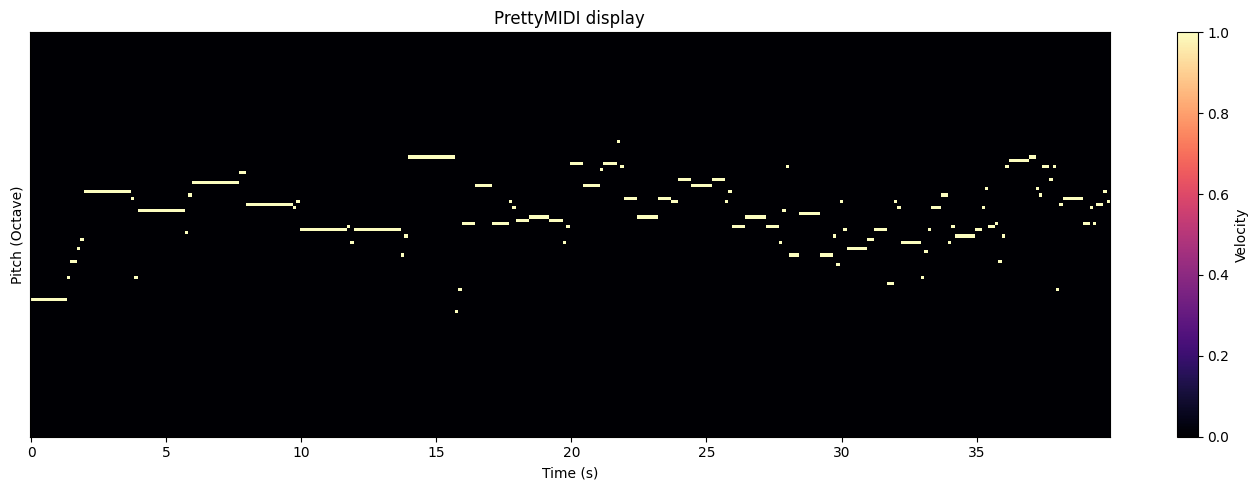
\includegraphics[width=\linewidth]{images/output_generated_2.png}
        \caption{Sample 2 generated by our final PianoGAN model.}
        \label{fig:output_generated_2}
    \end{subfigure}
    \caption{Visual comparison between real and generated piano rolls. The model successfully captures the rhythmic density and the chordal structure defined by the input conditioning.}
    \label{fig:output_comparison}
\end{figure*}


To obtain this result, we used one of the test samples from MAESTRO dataset and progressively produced 20 bars of music, each conditioned on the previously generated bar and on the underlying chord provided by the specific piece of music.
The result is a music that seems to really be conditioned on the underlying chord progression and previous bars, with no mode collapse or random note generation, as can be seen in Fig.~\ref{fig:output_comparison}.


% !TEX root = template.tex

\section{Concluding Remarks}
\label{sec:conclusions}

In this project we tried to tackle the problem of music generation by expanding the ideas already presented in \cite{Yang-2017}. We introduced a new way of setting the adversarial game, by using Wassersetin distance and gradient penalty instead of BCE loss. Furthermore, we gave a more profound structure to both the networks, providing them with a better understading of the music generation process.
We think that this network could be trained on different datasets and still be able to produce meaningful results, due to the various architectural constraints we imposed to the geneartion process.
However, we also think that longer trainings would be needed to fully understand how the network behaves and how different parameter tunings could lead to better results.

What we realised by designing this network is that it is difficult to understand how the different blocks interact with each other and hence how to improve the model.
However, we understood that cloesly analyzing the losses and the results are the most important factors in undesrtanding which are the required changes that should be made to the model.
Each block we added had its own purpose and we could only evaluate its effectiveness by looking at these data.

\bibliography{biblio}
\bibliographystyle{ieeetr}

\end{document}


